\subsubsection{Proton Background}\label{section:star_background_proton}
Secondary particles can be created due to the interaction of particles with detector dead-material.
The proton sample contains background from such protons knocked out  from the detector materials~\cite{STAR:spectra}. Most of these protons have large $DCA$ and are not reconstructed as primary particles. However, the rest with small $DCA$  are included in the primary track sample. Antiprotons do not have knockout background, hence the flat $DCA$ tail is almost absent from their $DCA$ distributions.

\begin{figure}[htpb]
	\centering
	\begin{subfigure}{.47\textwidth}
		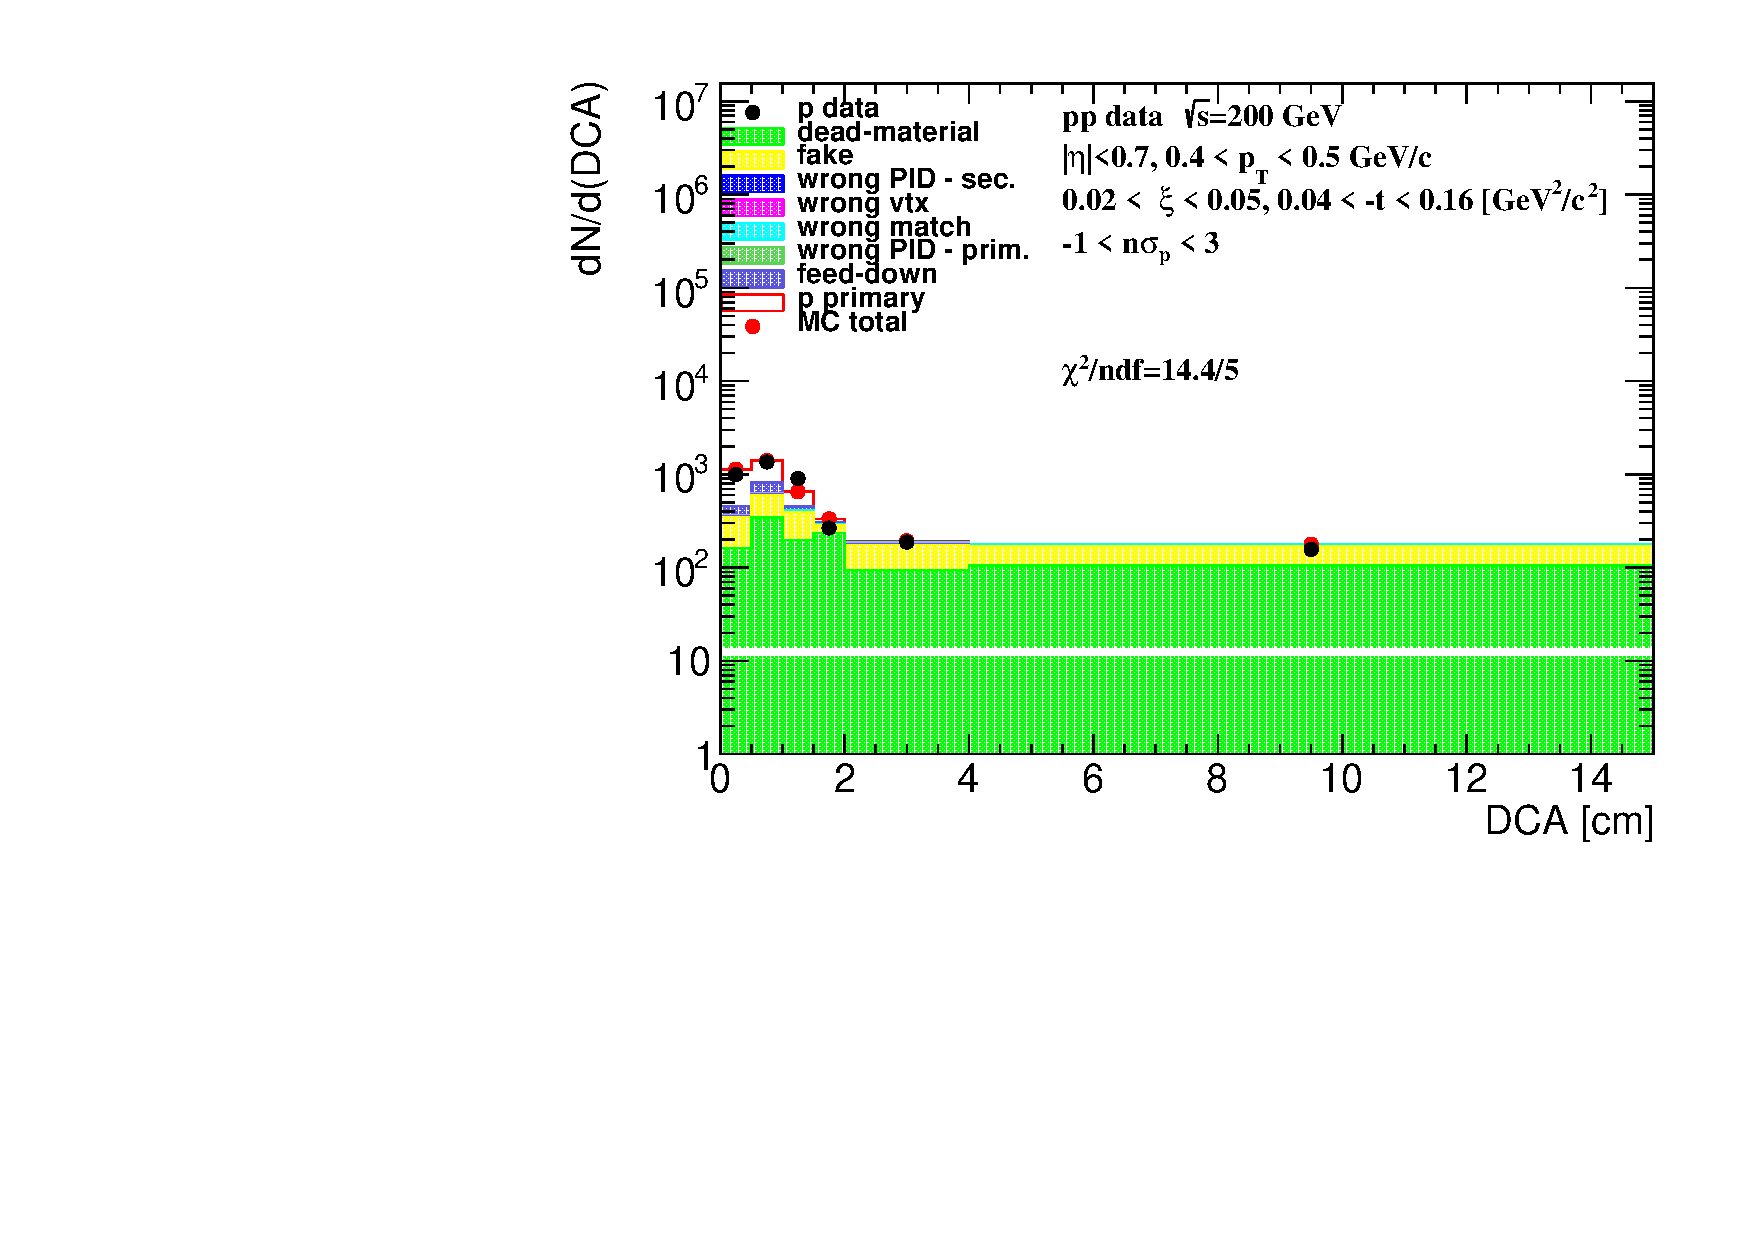
\includegraphics[width=\linewidth, page=1]{chapters/chrgSTAR/img/DCAproton/background_p_0.pdf}
	\end{subfigure}
	\begin{subfigure}{.47\textwidth}
		\includegraphics[width=\linewidth, page=2]{chapters/chrgSTAR/img/DCAproton/background_p_0.pdf}
	\end{subfigure}
	\begin{subfigure}{.47\textwidth}
		\includegraphics[width=\linewidth, page=3]{chapters/chrgSTAR/img/DCAproton/background_p_0.pdf}
	\end{subfigure}
	\begin{subfigure}{.47\textwidth}
		\includegraphics[width=\linewidth, page=4]{chapters/chrgSTAR/img/DCAproton/background_p_0.pdf}
	\end{subfigure}
	\caption[The $DCA$ distributions of protons for $0.4<p_T<0.5$~GeV/c shown for one range of $0.02<\xi<0.05$]{The $DCA$ distributions of protons for $0.4<p_T<0.5$~GeV/c shown for one range of $0.02<\xi<0.05$ (log and linear scale in left and right column, respectively). The MC  constributions are shown after scaling the dead-material template  to data. Background enriched samples were used in the normalization procedure (top), whereas the proton background was estimated from the nominal sample (bottom).}
	\label{fig:bkg_proton}
\end{figure}

In order to correct for the knock-out background protons, sample enriched in proton background  was used for background normalization, where $DCA_{xy}$, $DCA_z$ and $d_0$ cuts were abandoned. Additionally, at least one, instead of exactly one,  reconstructed vertex was required in this sample event selection.  Figure~\ref{fig:bkg_proton} and \ref{fig:bkg_proton_bar} shows the $DCA$ distributions of protons and antiprotons, respectively, for  nominal (bottom) and background enriched (top) samples. The protons and antiprotons are selected by a $dE/dx$ cut of $-1 < n\sigma_{p,\bar{p}} < 3$ where $n\sigma_{p,\bar{p}}$ is given by Eq.~\ref{eq:nsigma}. The fraction of knock-out proton within the selected sample is determined via a MC template normalization method. The templates of reconstructed tracks with $dE/dx$ of proton and antiproton were obtained from MC:
\begin{itemize}
	\item primary (anti)protons,
	\item knock-out background protons (labeled as \textit{dead-material}),
	\item fake tracks,
	\item secondary particles with $dE/dx$ of (anti)proton (labeled as \textit{wrong PID - sec.}),
	\item tracks associated to primary (anti)protons, but the reconstructed vertex is not matched to true-level primary vertex (labeled as \textit{wrong vtx}),
	\item reconstructed track is partially matched to true-level particle (labeled as \textit{wrong match}), i.e.  track and true-level particle have the appropriate number of common hit points but the distance between true-level particle and track is too large, $\delta^2\left(\eta,\phi\right)>\left(0.15\right)^2$,
	\item primary particles with $dE/dx$ of (anti)proton (labeled as \textit{wrong PID - prim.}),
	\item (anti)proton as a product of short-lived decays, mainly $\Lambda^0$ (labeled as \textit{feed-down}).
\end{itemize}

\begin{figure}[htpb]
	\vspace{-1cm}
	\centering
	\begin{subfigure}{.47\textwidth}
		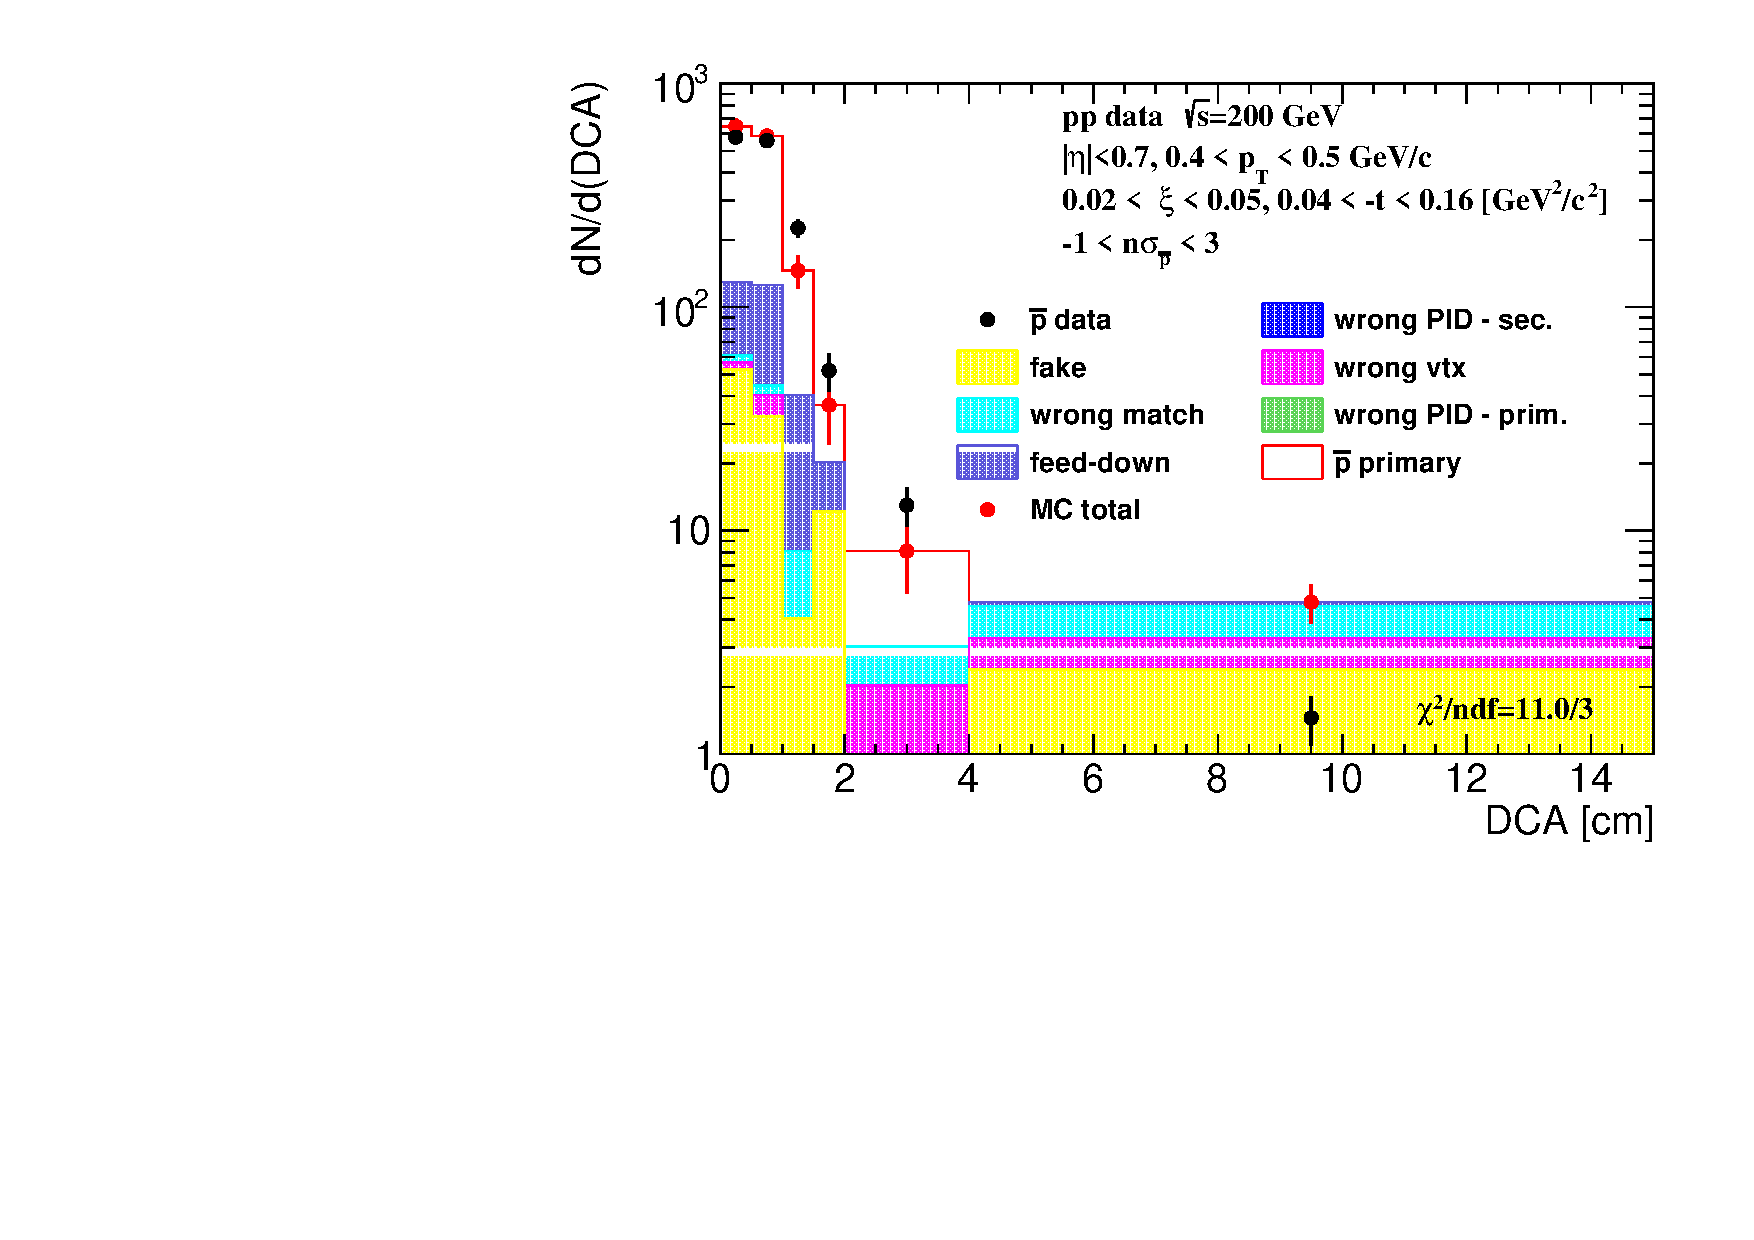
\includegraphics[width=\linewidth, page=1]{chapters/chrgSTAR/img/DCAproton/background_p_bar_0.pdf}
	\end{subfigure}
	\begin{subfigure}{.47\textwidth}
		\includegraphics[width=\linewidth, page=2]{chapters/chrgSTAR/img/DCAproton/background_p_bar_0.pdf}
	\end{subfigure}
	\begin{subfigure}{.47\textwidth}
		\includegraphics[width=\linewidth, page=3]{chapters/chrgSTAR/img/DCAproton/background_p_bar_0.pdf}
	\end{subfigure}
	\begin{subfigure}{.47\textwidth}
		\includegraphics[width=\linewidth, page=4]{chapters/chrgSTAR/img/DCAproton/background_p_bar_0.pdf}
	\end{subfigure}
	\caption[The $DCA$ distributions of antiprotons for $0.4<p_T<0.5$~GeV/c shown for one range of $0.02<\xi<0.05$]{The $DCA$ distributions of antiprotons for $0.4<p_T<0.5$~GeV/c shown for one range of $0.02<\xi<0.05$ (log and linear scale in left and right column, respectively). The MC controbutions are shown as colour histograms. Background enriched (top) and  nominal (bottom) samples were used.}
	\label{fig:bkg_proton_bar}
	%\vspace{-1cm}
\end{figure}

First, the background enriched sample was used  (Fig.~\ref{fig:bkg_proton}, top), where the template of knock-out background protons was normalized to the number of events in the fake-subtracted tail of the $DCA$ distribution, $3<DCA<15$~cm. Next the knock-out proton and fake background was subtracted from the $DCA$ distribution and the sum of other templates was normalized to the number of events in the signal region,  $DCA<1.5$~cm. 


The fraction of the knock-out proton background in the signal region, $DCA<1.5$, was estimated from the nominal sample (Fig.~\ref{fig:bkg_proton}, bottom), where $DCA_{xy}$, $DCA_z$ and $d_0$ track cuts were applied and exactly one reconstructed vertex was required. The normalization of each MC contribution was kept the same as that estimated for the background enriched sample. Figure~\ref{fig:bkg_proton_fit} shows the knock-out proton background as a function of $p_T$ in three ranges of $\xi$. The following functional form was found to describe the
background protons well:
\begin{equation}
f_{bkg}^{p}\left(p_T\right) = a_0\exp\left(a_1p_T\right)+a_2
\end{equation}
where  $a_k$, $k \in \mathbb N$, are fit free parameters. \\
\captionsetup{format=plain,indention=0pt,justification=justified}
\begin{wrapfigure}{r}{0.45\textwidth}
	\centering
	\vspace{-20pt}
	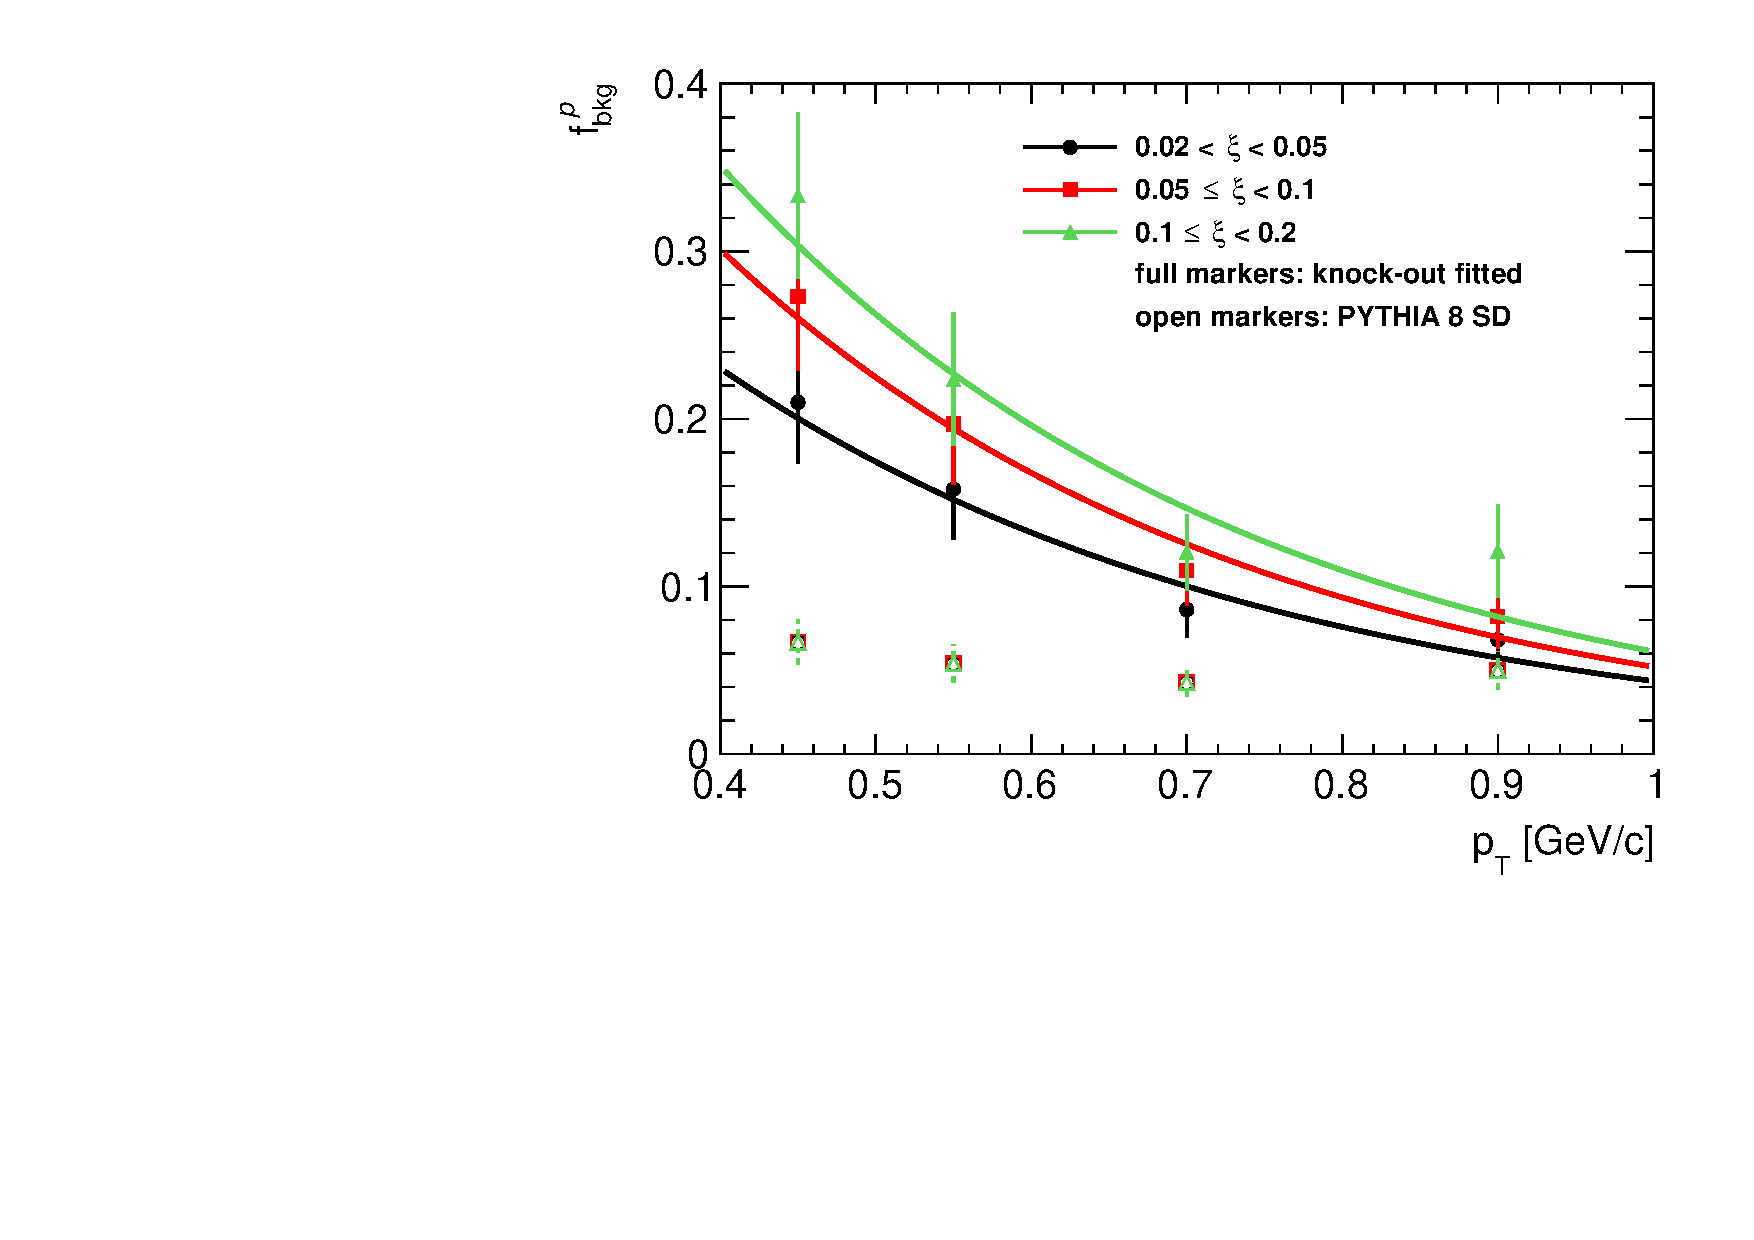
\includegraphics[width=\linewidth, page=1]{chapters/chrgSTAR/img/DCAproton/bkg_p.pdf}
	\vspace{-20pt}
	\caption{The fraction of knock-out proton background  as a function of $p_T$ in three ranges of $\xi$  with  fitted parametrizations.}
	\vspace{-80pt}
	\label{fig:bkg_proton_fit}
\end{wrapfigure}
 The obtained fraction of knock-out background protons is approximately $20\%$ at $p_T = 0.45$ GeV/c
 and less than $10\%$ at $p_T = 1.0$~GeV/c. The fraction of knock-out background protons depends on a number of factors, including the amount of detector material, analysis cuts and the $\xi$ of diffractive proton. 
 Figure~\ref{fig:bkg_proton_bar} shows the corresponding $DCA$ distributions with MC templates for antiprotons, where the background form knock-out particles is not present. The MC templates  fairly well describe the $DCA$ distribution for both, protons and antiprotons. Additionally, there is a small $\left(<1\%\right)$ background  contribution, present for both particles, which also was taken into account and subtracted. It originates from reconstructed tracks which have the appropriate number of common hit points with true-level particle, but the distance between them is too large, i.e. $\delta^2\left(\eta,\phi\right)>\left(0.15\right)^2$.
 \captionsetup{format=default,indention=0pt,justification=justified}
 \FloatBarrier